\documentclass[12pt]{article}
\usepackage{indentfirst}
\usepackage{amsmath}
\usepackage{multicol}
\setlength{\jot}{2ex}
\usepackage{mathrsfs}
\usepackage{graphicx}
\usepackage{wrapfig}
\usepackage{booktabs}
\usepackage[letterpaper, margin=1in]{geometry}
\usepackage{fancyhdr}
\usepackage{enumitem}
\usepackage[autostyle, english = american]{csquotes}
\MakeOuterQuote{"}
\renewcommand{\baselinestretch}{1.0}
\newcommand{\objects}[2]{%
  \leavevmode\vbox{\hbox{#1}\nointerlineskip\hbox{#2}}%
}
\title{Lab 1 \\ The RC Series Circuit}
\author{Qadis Chaudhry}
\date{October 16, 2021}
\begin{document}
\maketitle
    \section*{Introduction}
    \par The purpose of the experiments within this lab, is to observe the behavior of the resistor-capacitor circuit and mainly how changes in the source voltage are translated to the voltage across the capacitor. There are two main responses that need to be examined when dealing with the RC circuit, the natural response and the step response. The natural response is where the capacitor has been charged initially and is connected across with a resistor which allows the capacitor to discharge. The step response is where the capacitor is charged via a source. These responses can be achieved by connecting a capacitor and a resistor in parallel along with a source with a switch.
    \par With this configuration, when the switch is connected, the capacitor is able to charge and given enough time, it will charge up to where the voltage across the capacitor is equal to the voltage of the source. The connection of the source will yield a step in the voltage across the capacitor since the voltage in the circuit will jump instantaneously from zero up to whatever the source value is. For this reason, this response is known as the step response of the RC circuit. This response will also be seen with the connection of a square input source function for the voltage. The source voltage going from the negative peak to the peak value will be equivalent to connecting the switch in the circuit.
    \par With the same configuration, once the capacitor is charged, the switch can be disconnected and this will initiate the natural response of the RC circuit. The capacitor will discharge slowly as it flows through the resistor and eventually equalizes. This discharging can be seen with the connection of the multimeter across the capacitor and if we plot these decreasing values as a function of time, we will see a non-linear decreasing function representing the discharge. This curve can be linearized by using the properties of logarithms and the slope of this line will be equal to the negative inverse of the time constant of the circuit.
    \par The last aspect of this circuit that we can examine is its ability to preform integration and differentiation. If we have a circuit where the resistor and capacitor are connected in series, the loop of voltage can be described as the individual voltages across each of the elements, set equal to zero. If we observe the equation for the voltage across a capacitor we can see that it is an integral, and with some manipulation, we get an expression which approximates the integration of the input source voltage.
    \newpage
    \section*{Prelab Exercises}
    \begin{itemize}
        \item[3.2]
            Since the time constant $\tau=RC$, where $R=1\ M\Omega$ and $C=100\ \mu F$,
            \begin{align*}
                \tau &= (1 \times 10^{6})(100 \times 10^{-6}) \\
                \tau &= \boxed{100\ s}
            \end{align*}
        \item[3.4]
            \par With the connection of the series RC circuit, we can approximate the integral or the derivative of the source voltage.  If we look at the loop of the voltage within this circuit it will be,
            \[
                v(t) = v_C(t) + v_R(t)
            \]
            If the voltage across the capacitor is not very large, the source voltage can be approximated to be equal to the voltage across the resistor, since $v_C \approx 0$. This can be done by making the period of the source function a lot smaller than the time constant which will cause the capacitor to not be able to charge up to a significant amount, keeping the condition of $v_C$ being very small true. If this is the case, we can examine the voltage across the capacitor,
            \[
                v_C(t) = \frac{1}{C} \int i(t)\ dt
            \]
            and see that since this is a series circuit, the current flowing through both of the elements will be the same. If we divide this equation by the $R$, we can get the integral for the resistor voltage,
            \[
                \frac{1}{C} \int \frac{i(t)}{R}\ dt \approx \frac{1}{RC} \int v_R(t)\ dt
            \]
            From this, we can see that since $RC = \tau$, and we said initially that the case was such that $v(t) \approx v_R(t)$,
            \[
                v_C(t) \approx \frac{1}{\tau} \int v(t)\ dt
            \]
            For differentiation, the concept is the same instead only this time, the period of the function needs to be very large since after long periods of time, the voltage across a capacitor resembles the voltage of the source. Following the same process as before only this time starting with the resistor voltage,
            \[
                v_R(t) = R i(t) = R C \frac{d v_C(t)}{dt}
            \]
            and since $\tau = RC$ and after a long time $v_C(t) \approx v(t)$,
            \[
                v_R(t) \approx \tau \frac{d v(t)}{dt}
            \]
    \end{itemize}
    \newpage
    \section*{Experiments and Results}
    \begin{figure}[h]
        \centering
        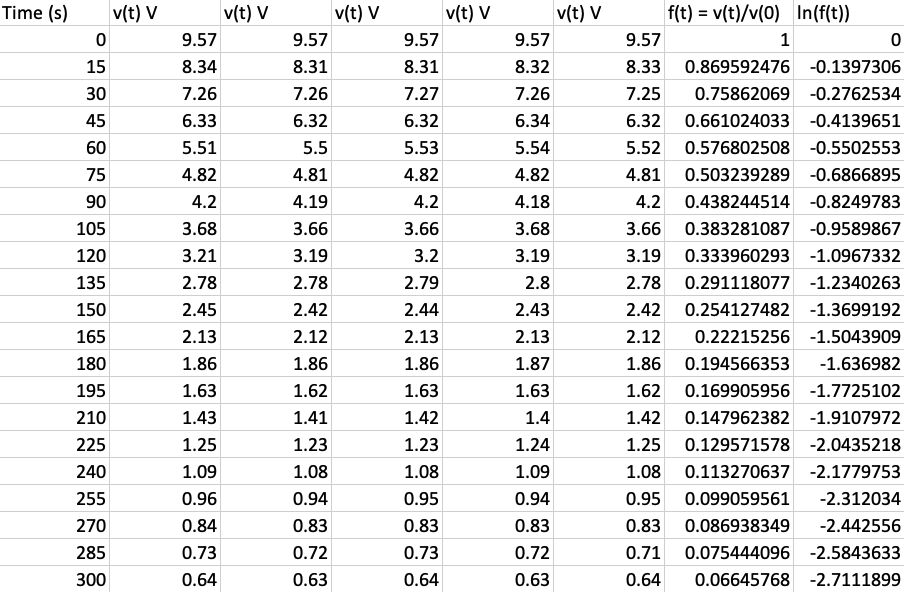
\includegraphics[width=0.75\textwidth]{Data Table.png}
    \end{figure}
    \begin{center}
        Figure 1: Voltage Data Table
    \end{center}
    \begin{figure}[h]
        \centering
        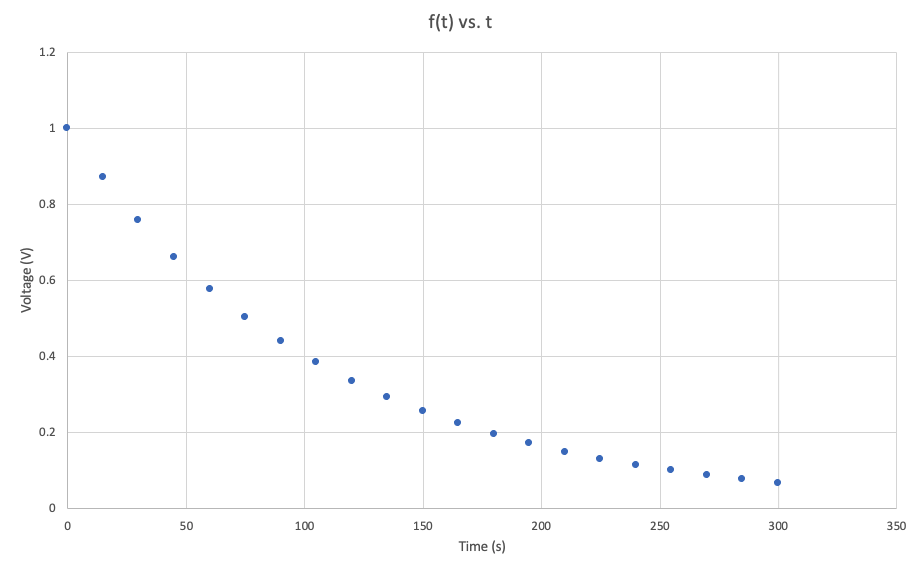
\includegraphics[width=0.8\textwidth]{5.1 Graph 1.png}
    \end{figure}
    \begin{center}
        Figure 2: Graph of $f(t)$
    \end{center}
    \newpage
    \noindent 5.1
    \begin{itemize}
        \item[(a)]
            From the graph we can get the value of $\tau$ by determining at what time $t$ the graph of $f(t) = f(0)e^{-1}$. Since the value of $f(0)$ equals 1, we just need to find the time for which the function is equal to $e^{-1}$. This can be approximated by finding the equation of a line connecting two points close to this value, and then using that line to find the value of $t$ which makes the equation true. We can see that the two closest values to $e^{-1}$ are, (105, 0.383) and (120, 0.334). To find the equation of the line between these points we must find the slope using the slope formula,
            \[
                \frac{y_2 - y_1}{x_2 - x_1} = \frac{0.334 - 0.383}{120 - 105} =
                \frac{-0.49}{15} = -0.0032667
            \]
            Using this we can write the equation for $f(t)$ over this small interval,
            \[
                f(t) = -0.0032667 t + b
            \]
            To find $b$ we can use one of the points,
            \[
                0.383 = -0.0032667 (105) + b
            \]
            \[
                b = 0.383 + 0.0032667(105) = 0.726
            \]
            This makes the final equation for that interval,
            \[
                f(t) = -0.0032667 t + 0.726
            \]
            From here we can plug $e^{-1}$ into the equation to find the value of $t$ which makes this true.
            \[
                e^{-1} = -0.0032667 t + 0.726
            \]
            \[
                t = \frac{e^{-1} - 0.726}{-0.0032667} = 109.6287
            \]
            Since this value of $t$ is the time constant, we complete the statement as,
            \[
                \boxed{\tau = 109.6287\ s}
            \]
    \end{itemize}
    \newpage
    \begin{figure}[h]
        \centering
        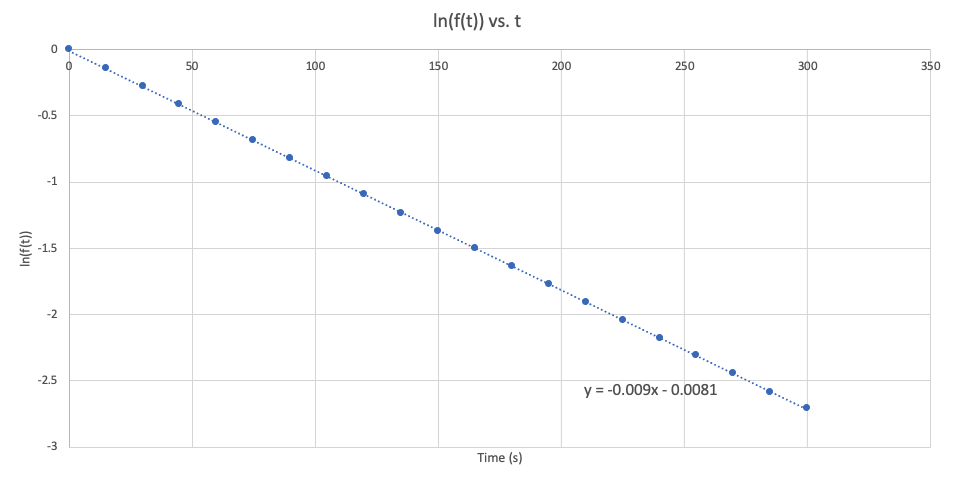
\includegraphics[width=0.8\textwidth]{5.1 Graph 2.png}
        \caption{Graph of $\ln(f(t)) \text{ vs. } t$}
    \end{figure}
    \begin{itemize}
        \item[(b)]
            Shown above is the graph of the natural logarithm of the function $f(t)$, plotted against time. Since $f(t)$ is technically some decaying exponential of the form,
            \[
                f(t) = A e^{t / \tau}
            \]
            taking the natural logarithm of both sides we get,
            \[
                \ln(f(t)) = (-1 / \tau) t + \ln(A)
            \]
            From this we can see that it is a linear equation of the form, $y = mx + b$. If we are to graph $\ln(f(t))$ versus time, as we have above, the negative inverse of the slope of the line will result in the value for $\tau$, the time constant. We can see from the graph that the program has generated a trend line for the plotted point.  The slope of this trend line is,
            \[
                m = -0.009 = -1 / \tau
            \]
            Taking the negative inverse of this will yield $\tau$:
            \[
                \tau = -(-0.009)^{-1} = \frac{-1}{-0.009} = \boxed{111.111\ s}
            \]
    \end{itemize}
    \noindent 5.2
    \begin{itemize}
        \item[(a)]
            Using the information provided, we know that of a complete curve of $ f(t) $ will yield be equal to $ A\tau $. Now, to find the value of $ A $ we can use the equation and graph utilized in the previous part,
            \[
                \ln(f(t)) = (-1 / \tau)t + \ln(A)
            \]
            From the equation of the trend line for the graph we can find the value of $ A $ to be,
            \[
                \ln(A) = -0.0081
            \]
            \[
                A = e^{-0.0081} = 0.99193
            \]
            Using this we can find the value of $ \tau $ since from the equation of the area under the curve since,
            \[
                \int_0^\infty f(t)\ dt = A \tau
            \]
            \[
                \tau = \frac{\int_0^\infty f(t)\ dt }{A}
            \]
            Using the program to commute the area under the curve with the trapezoidal rule we get that the area is equal to 102.63166. From this, we can find the value of $ \tau $ by taking this value and dividing by the value of $ A $,
            \[
                \tau = \frac{102.63166}{0.99193} = \boxed{103.4647\ s}
            \]
            This answer for $ \tau $ here is further from the other approximations and this is due to the fact that we do not have a complete curve of $ f(t) $. This causes the assumption for the area under the curve being equal to $ A\tau $ inaccurate to certain degree, throwing off the value of $ A $ and therefore, the value of $ \tau $.
        \item[(b)]
            The trapezoidal rule can be used to approximate the area under a curve. The equation is given and the variables can be defined plugged in to give a value of $ \tau $. Here, $ \Delta t = 15$ since each of the values of the function $ f(t) $ were taken 15 seconds apart. The rest of the variables can be taken from the table as, $ f_1 = 1 $, $ f_{n} = 0.06645768 $, and $ N = 20 $. The Sigma term will just be the sum of the values ranging from $ f(2) $ to $ f(20) $.  This gives the final equation being,
            \[
                \tau = 15 \left( \frac{1+0.06645768}{2} + \sum_{i=2}^{N-1} f_{i} \right)
            \]
            \[
                \tau = \boxed{102.63166\ s}
            \]
    \end{itemize}
    \noindent 5.3
    \par The given formula can be used to find the approximate value of $ \tau $ since this is the definition of a derivative. The term $ f(t_0 + \Delta t) $, will just be the next value of $ f(t) $ after $ f(t_0) $. Using this information, the equation can be applied to three different points and the value of $ \tau $ can be attained as an average of the three values.
    \begin{align*}
        \tau_1 &= f(2) \frac{15}{f(2) - f(3)} = 116.595 \\
        \tau_1 &= f(8) \frac{15}{f(8) - f(9)} = 116.927 \\
        \tau_1 &= f(13) \frac{15}{f(13) - f(13)} = 116.143
    \end{align*}
    \[
        \tau_{avg} = \frac{116.595 + 116.927 + 116.143}{3} = \boxed{116.555\ s}
    \]
    \newpage
    \noindent 5.4
    \begin{figure}[h]
        \centering
        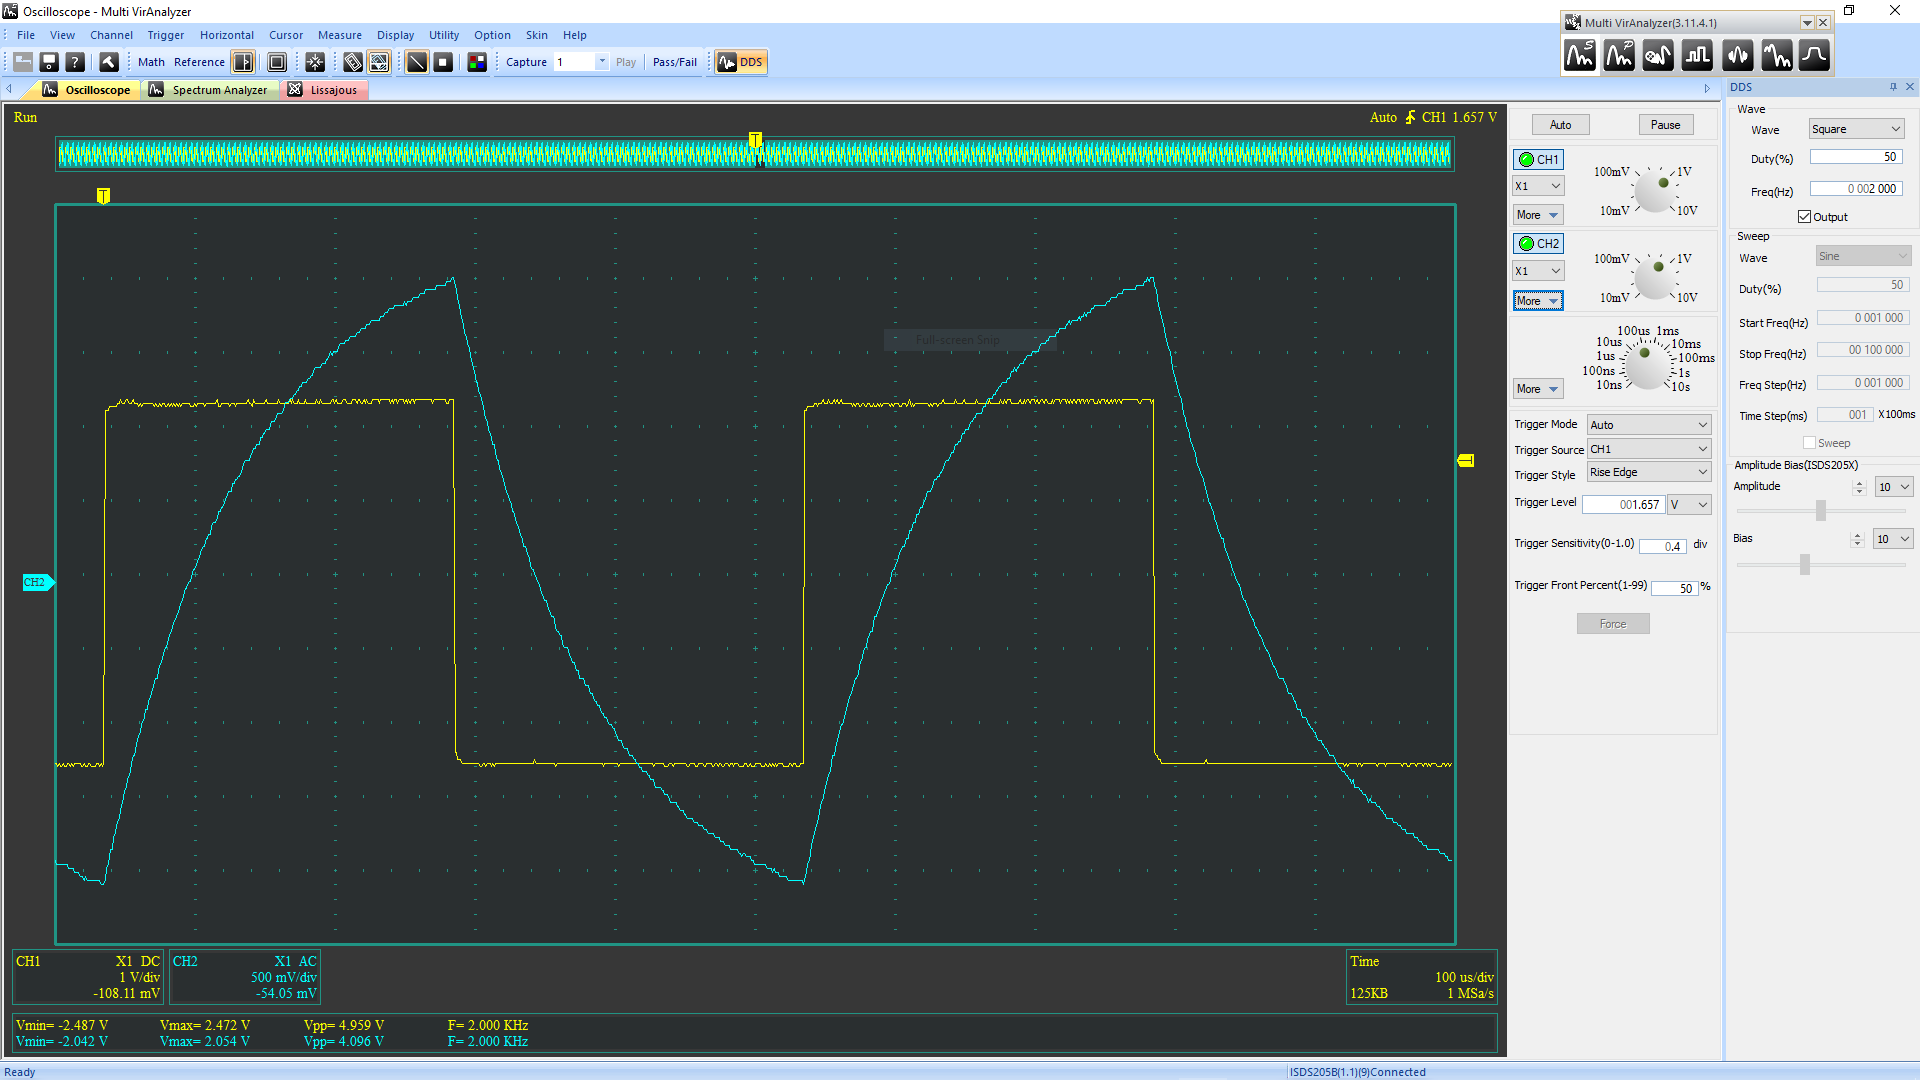
\includegraphics[width=\textwidth]{4.2 f.png}
        \caption{Waveform for part 4.2 f}
    \end{figure}
    \par From the waveform we can see the measured values of $ V_{pp} $ and $ V_{cpp} $.
    \[
        \frac{V_{pp}}{V_{cpp}} = \frac{4.959}{4.096} = 1.2107
    \]
    Given the equation,
    \[
        V_{cpp} = V_{pp} \left( 1-e^{-A} \right) \left( 1+e^{-A} \right)
    \]
    we can find the value of $ V_{pp} / V_{cpp} $ and compare to the one found from the waveform, the value of $ A $ being the one found in the previous parts.
    \begin{align*}
        \frac{V_{pp}}{V_{cpp}} &= \left( \left( 1-e^{-A} \right) \left( 1+e^{-A} \right) \right)^{-1} \\
                               &= \left( \left( 1-e^{-0.99193} \right) \left( 1+e^{-0.99193} \right) \right)^{-1} \\
                               &= 1.1597
    \end{align*}
    From this it can be seen that the theoretical value and the measured value are significantly close to one another and performing a percent error calculation,
    \[
        \%\ error = \frac{1.2107 - 1.1597}{1.1597} \times 100 = 4.397\ \%
    \]
    the error is under 5\% which means that the data is fairly accurate.
    \newpage
    \noindent 5.5
    \begin{center}
        \objects
            {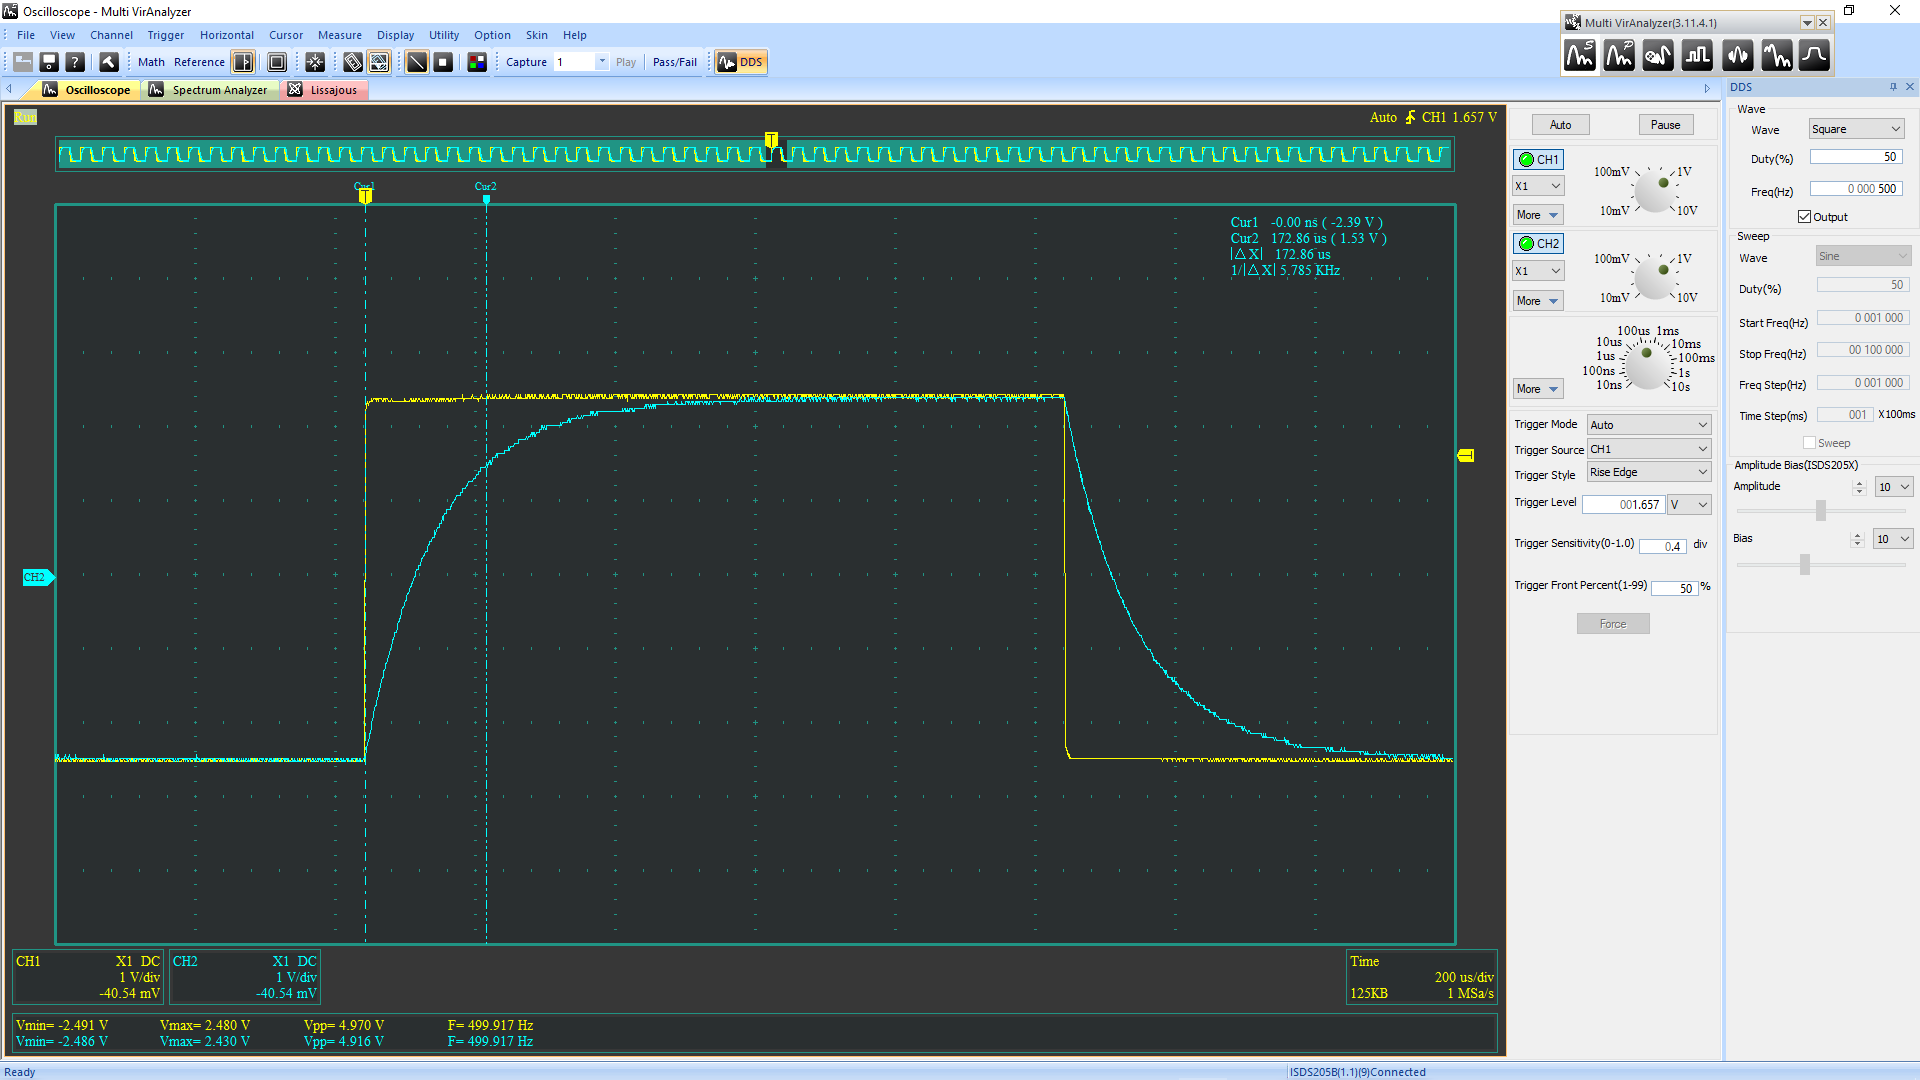
\includegraphics[width=0.95\textwidth]{4.2.png}}
            \,
            Waveform for part 4.2
            {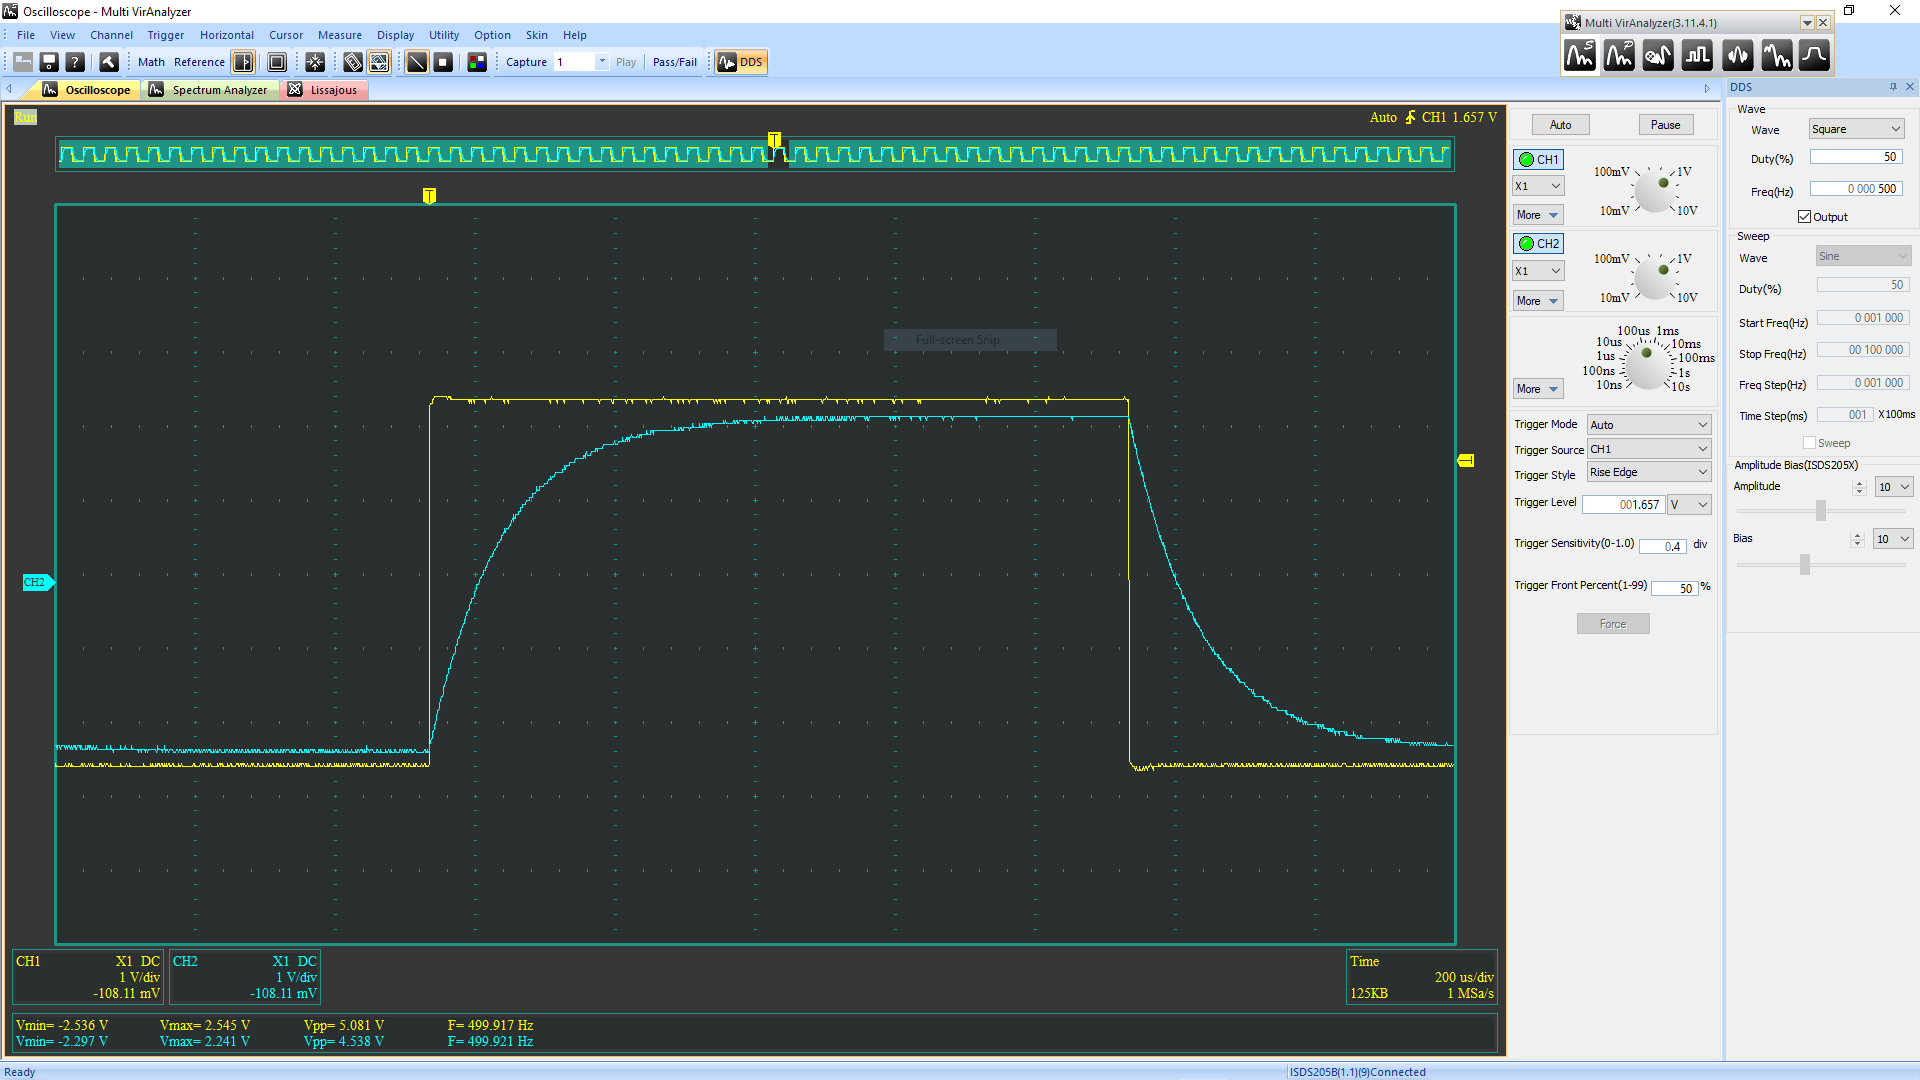
\includegraphics[width=0.95\textwidth]{4.2 d.png}}
            \,
            Waveform for part 4.2 d
    \end{center}
    \begin{center}
        The top waveform here is for part 4.2 and the bottom for part 4.2 d.  Originally for part 4.2, the circuit is created with a resistor value of 10 $ k\Omega $. For part d of this problem, the resistor is increased and the capacitor is decreased by a factor of ten, making the value of the resistor $ 100\ k\Omega $ and the value of the capacitor, $ 0.001\ \mu F$, or $ 1\ nF $.  It can be seen how the amplitude of the wave of the second image is slightly lower however, the waveforms are almost identical due to the time constant being identical.
    \end{center}
    \begin{center}
        \objects
            {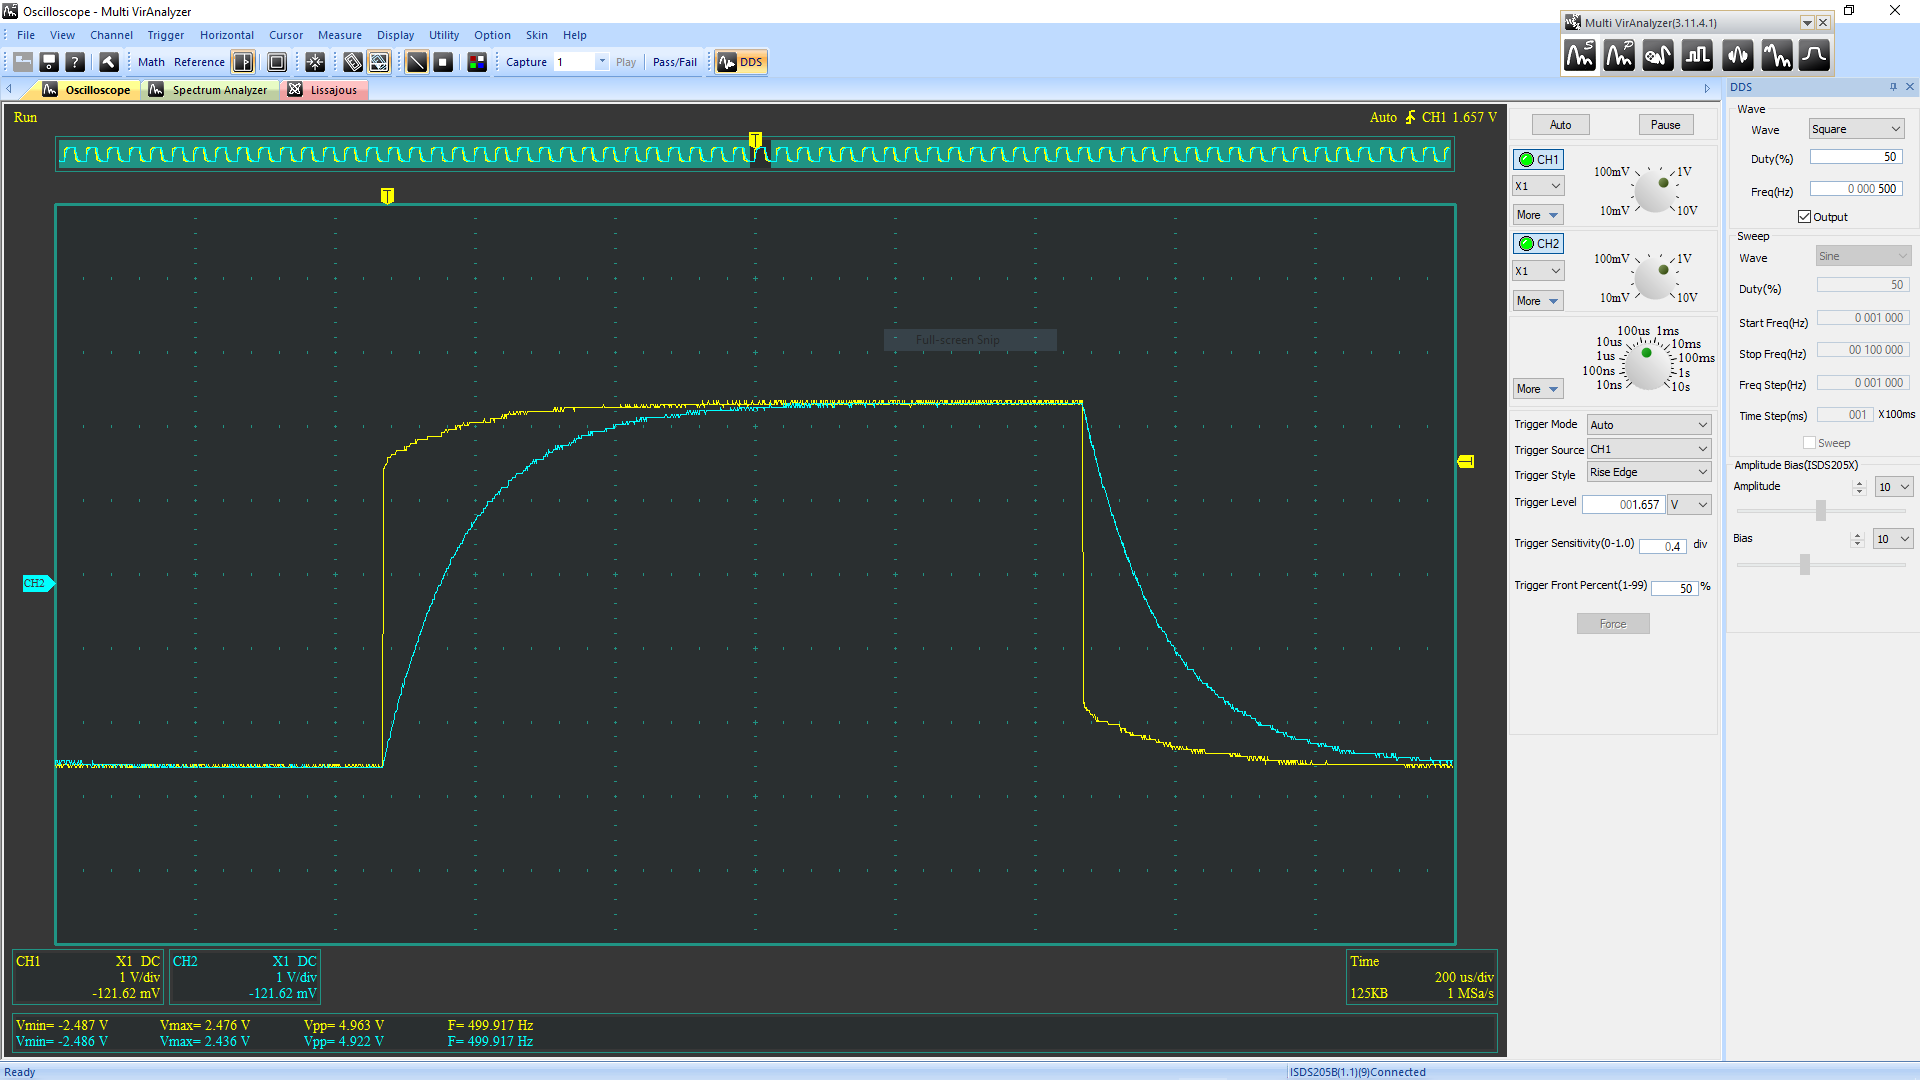
\includegraphics[width=0.95\textwidth]{4.2 e.png}}
            \,
            Waveform for part 4.2 e
            {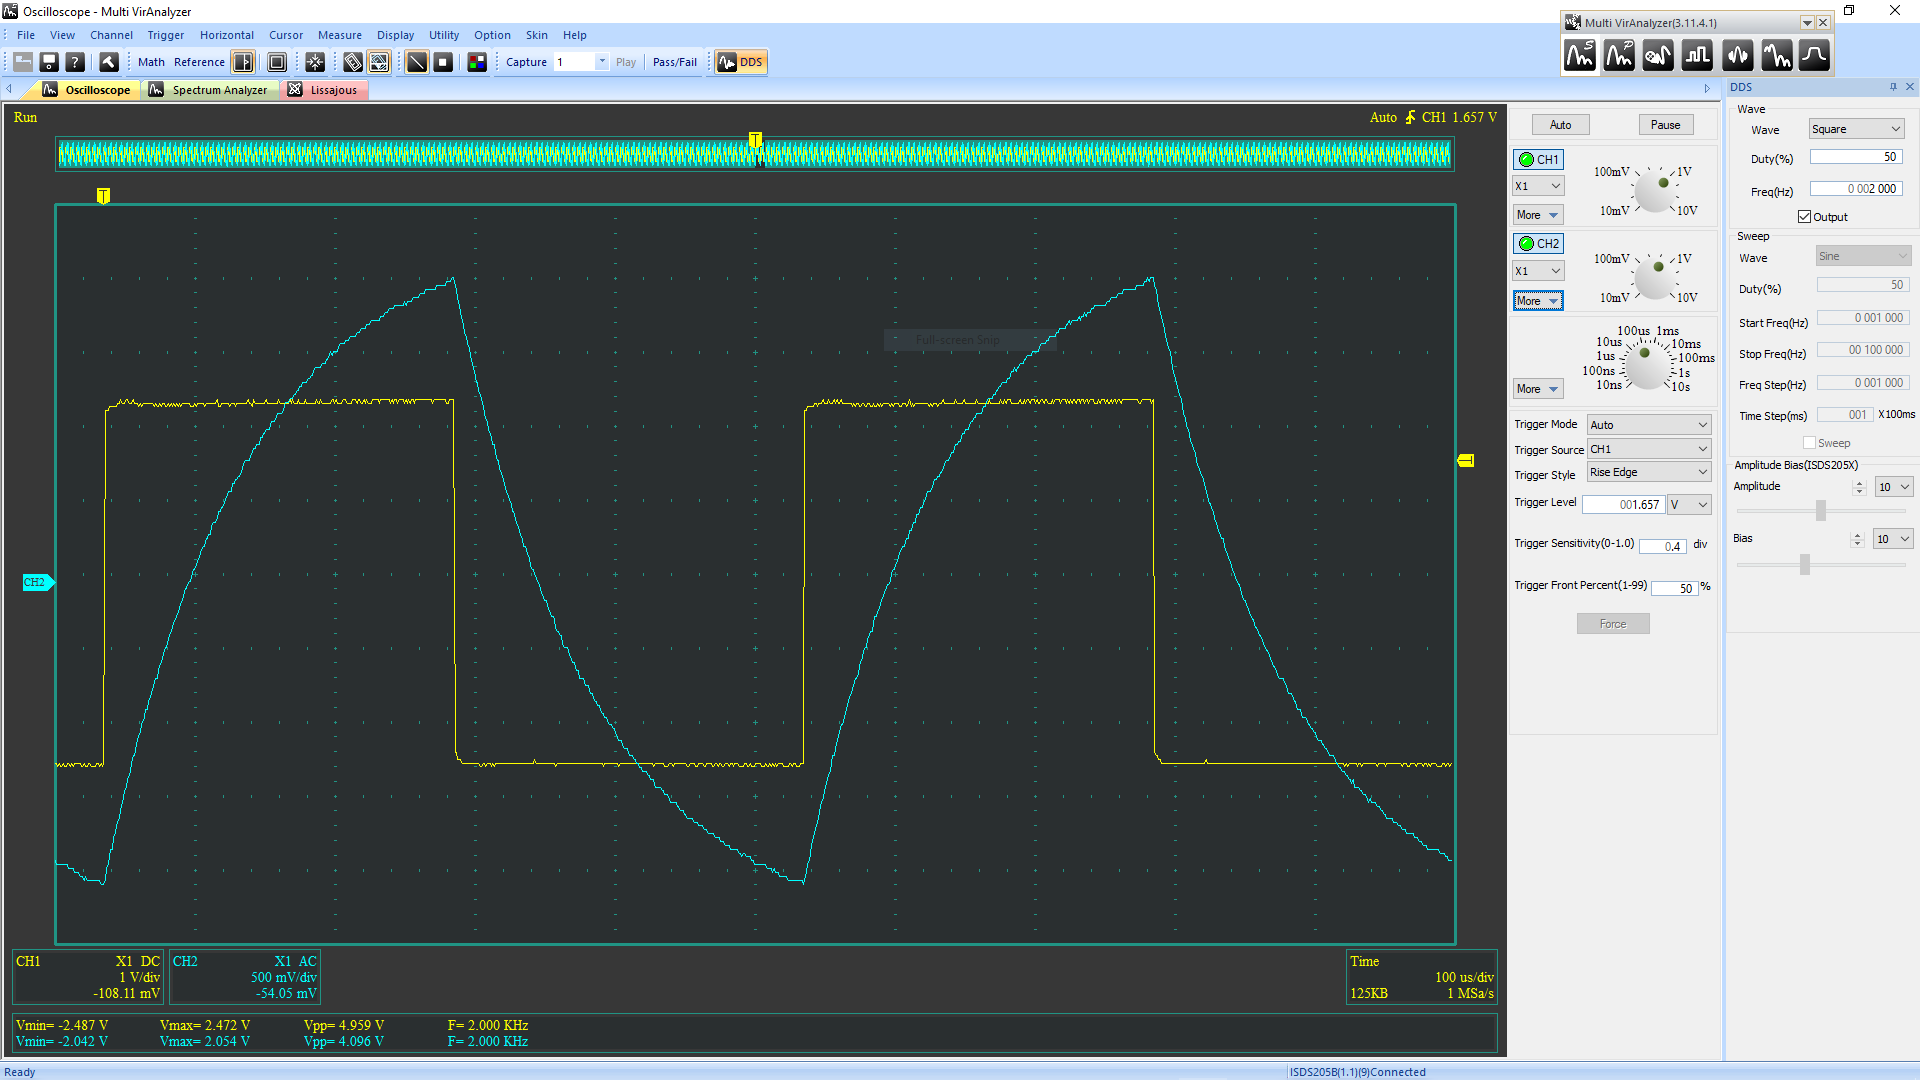
\includegraphics[width=0.95\textwidth]{4.2 f.png}}
            \,
            Waveform for part 4.2 f
    \end{center}
    \begin{center}
        Here we have the waveform for part 4.2 e on top and 4.2 f on the bottom.  For 4.2 e, the resistor value is decreased this time and the capacitor value is increased by a factor of ten. The value of the resistor in this case is $ 1\ k\Omega $ and the capacitor is $ 0.1\ \mu F $. The waveform is essentially the same as the default case in 4.2 since the time constant is the same. The waveform on the bottom is shown as the input frequency is raised from 50 Hz to 2 kHz. The time constant is 2.5 $ \tau $ so the curves are shifted and contracted horizontally. The peak voltage of the capacitor is 4.096 V.
    \end{center}
    \newpage
    \noindent 5.6
    \begin{figure}[h]
        \centering
        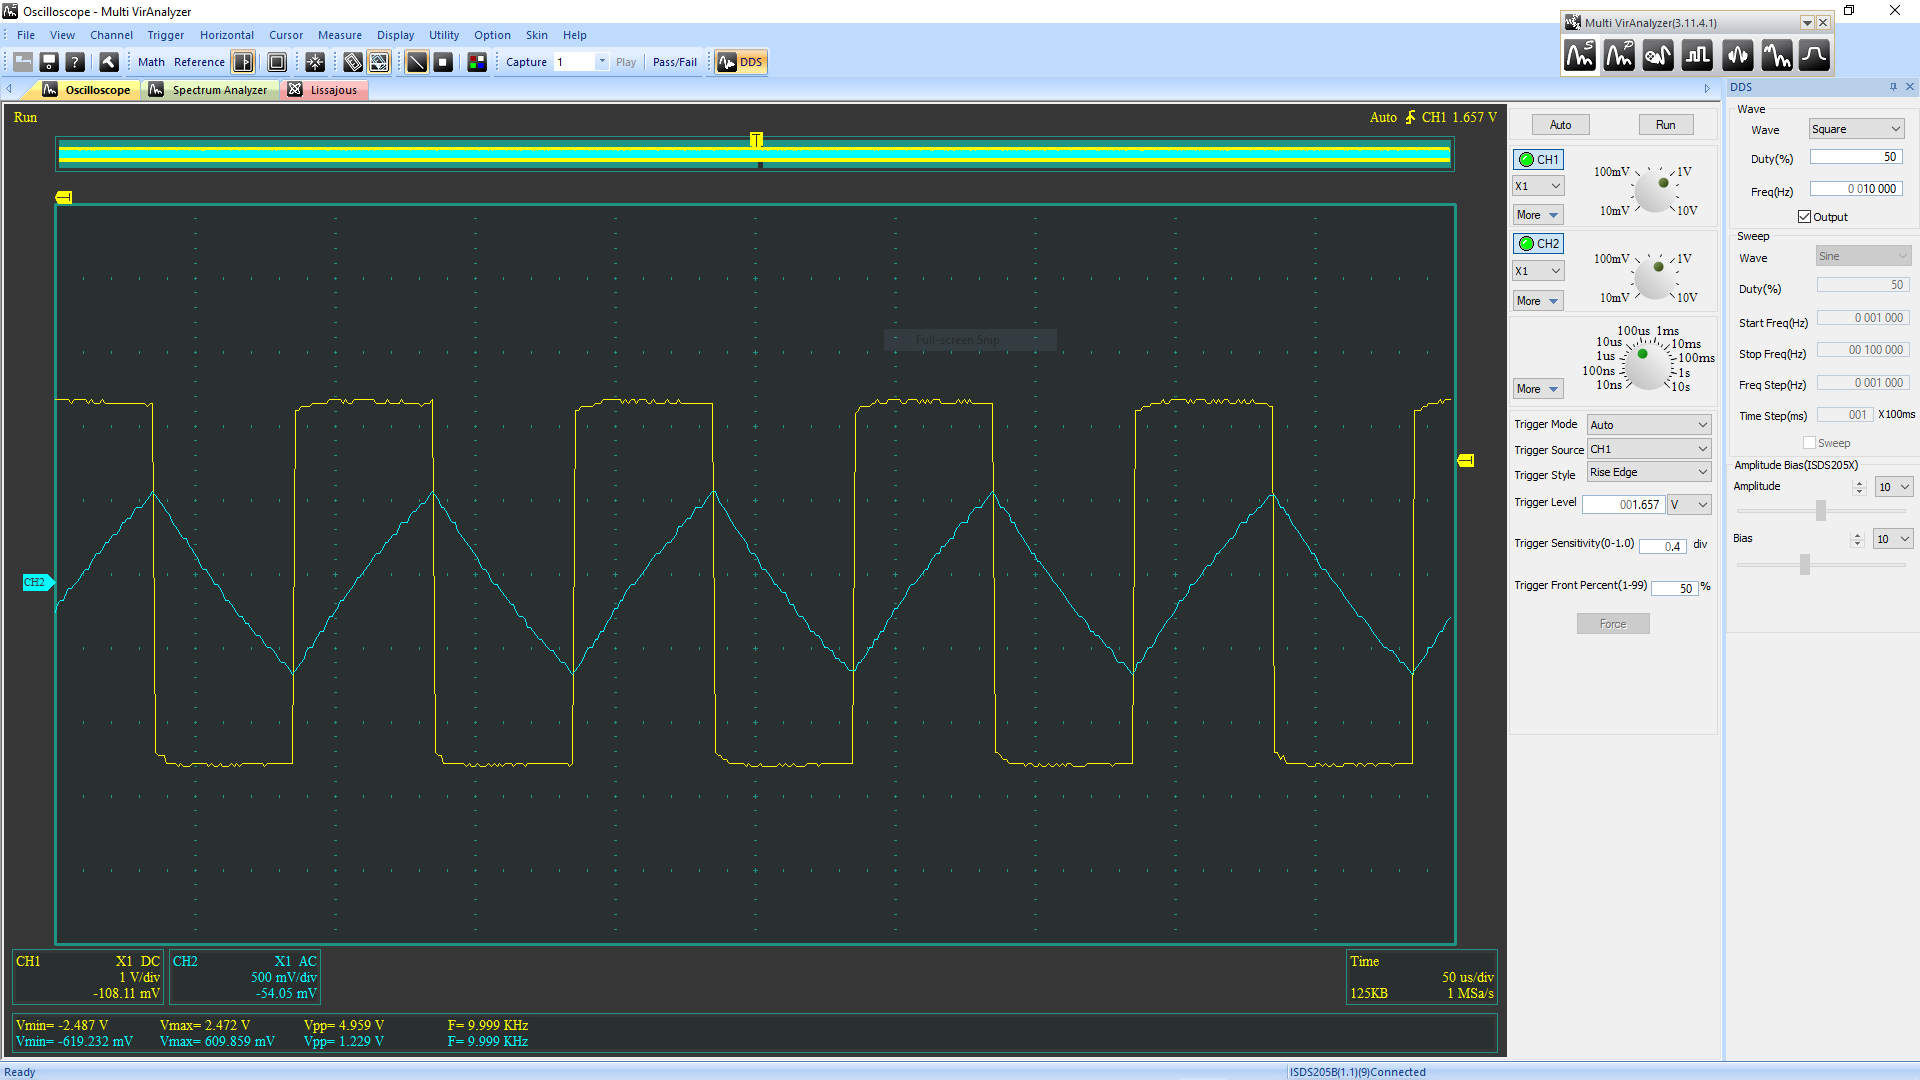
\includegraphics[width=\textwidth]{4.3.1.png}
        \caption{Waveform for part 4.3.1}
    \end{figure}
    \par This is the waveform for the integration circuit of a square input wave. To achieve behavior, the input frequency had to be raised until the output resembled the integral of a square wave, a triangle wave. This is the case at a frequency of 10 kHz which can be seen in the top right of the image. This is the minimum frequency at which the integrator serves its function and since the period is equal to the inverse of frequency, we can simply multiply this value by $ \tau $, which equals $ RC $ where $ R $ is $ 10\ k\Omega $ and $ C $ is $ 0.01\ \mu F $, to get the ratio $ \tau / T $.
    \[
        \frac{\tau}{T} = (10000)(10 \times 10^{3})(0.01 \times 10^{-6}) = 1
    \]
    The minimum ratio of $ V_{pp} / V_{cpp} $ can be seen from the measurements of the oscilloscope as being,
    \[
        \frac{V_{pp}}{V_{cpp}} = \frac{4.959}{1.229} = 4.035
    \]
    This value is 3.5 times the theoretical value achieved through the use of the equation, which is mainly due to the fact that the theoretical value was calculated at a frequency of 500 Hz rather the 10 kHz here.
    \newpage
    \noindent 5.7
    \begin{figure}[h]
        \centering
        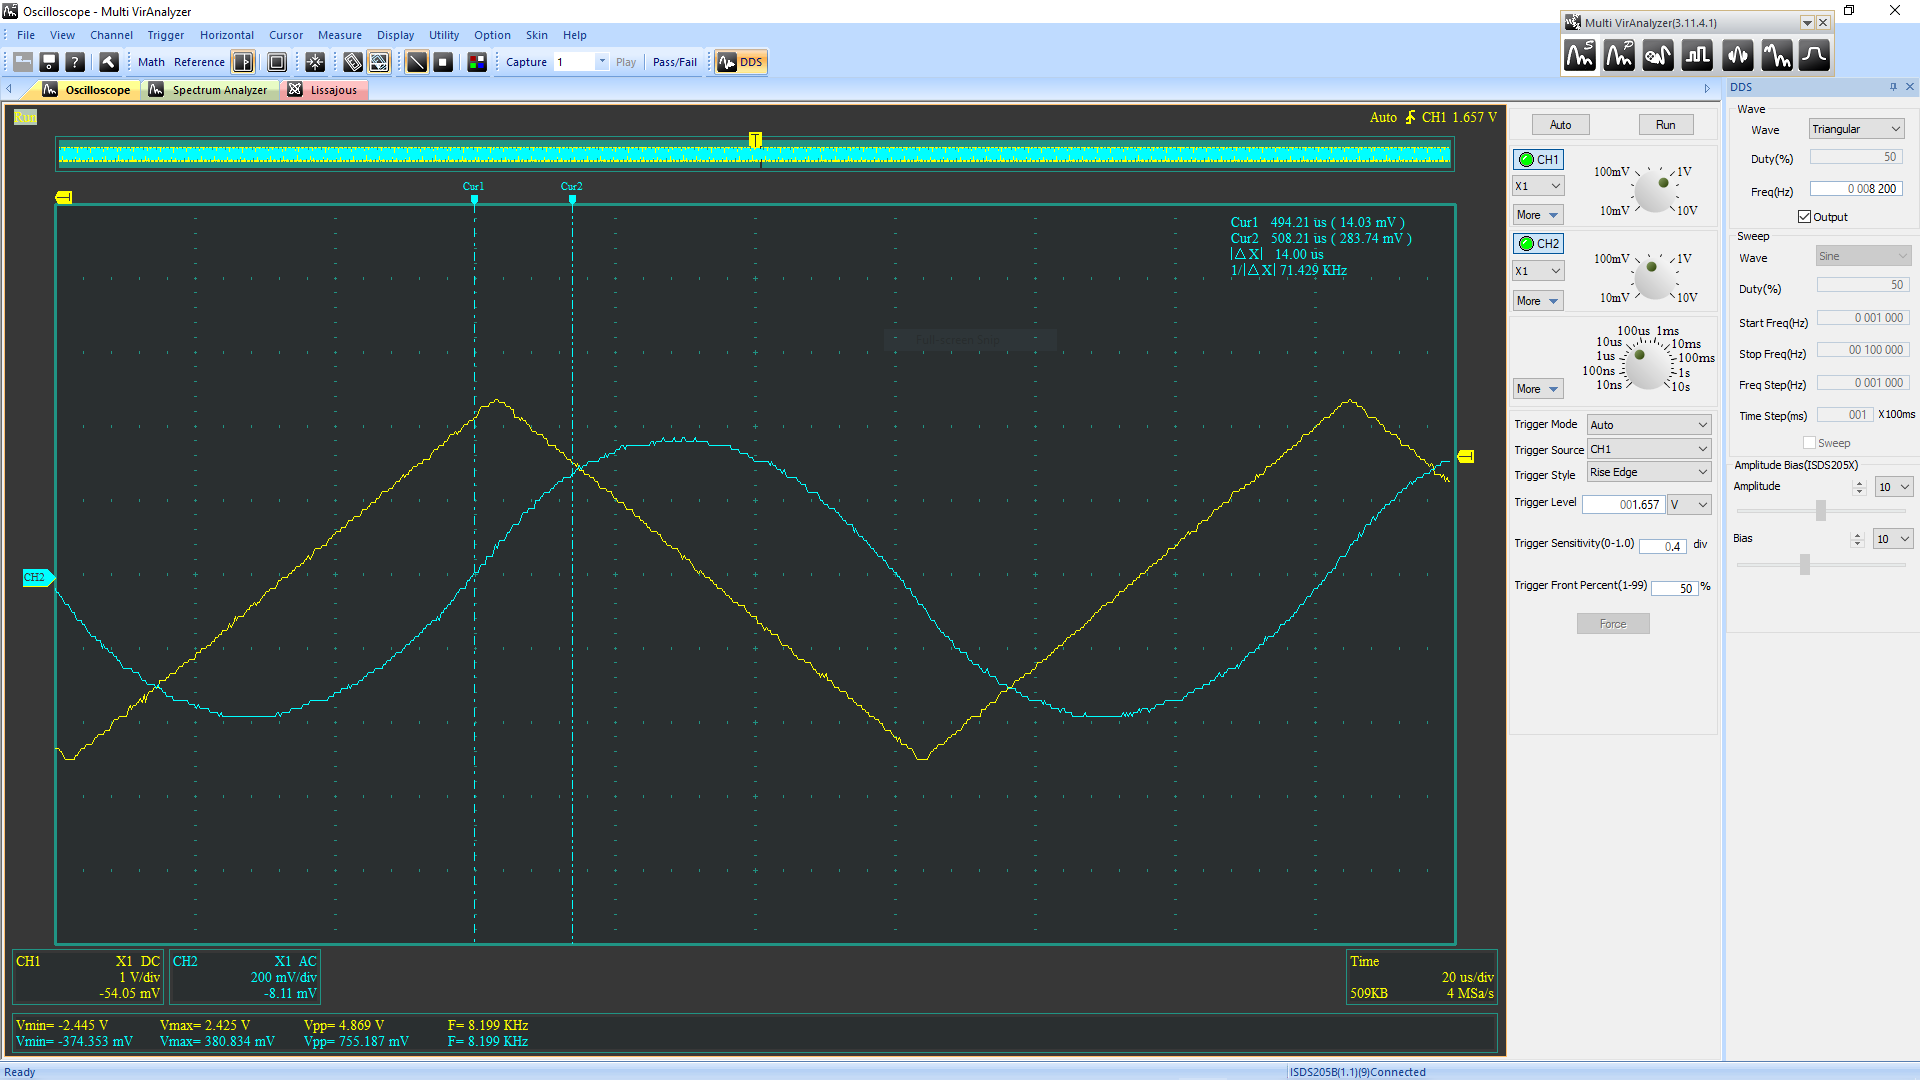
\includegraphics[width=\textwidth]{4.3.2.png}
        \caption{Waveform of part 4.3.2}
    \end{figure}
    \par Here we can see that the integration of a triangular wave is a curve which looks to be sinusoidal however, is parabolic in actuality. To show this we can take the value of $ V_{max} $ and multiply it by 3/4, and if this value is equal to that of the curve at 1/8 of its period, the curve is parabolic. In the image, the cursors are set so that one of them is at exactly 1/8 times the period of oscillation. The value for the voltage at this point is 283.74 mV. The value of the peak of the wave, $ V_{max} $ can also be seen and has a value of 380.834 mV. If the value of $ V_{max} $ is equal to 283.74, then this curve is indeed parabolic,
    \[
        V_{max} \times \frac{3}{4} = 285.63\ \text{mV}
    \]
    From this we can see that the values of are basically the same leading us to the conclusion that this curve is indeed parabolic.
    \newpage
    \noindent 5.8
    \begin{figure}[h]
        \centering
        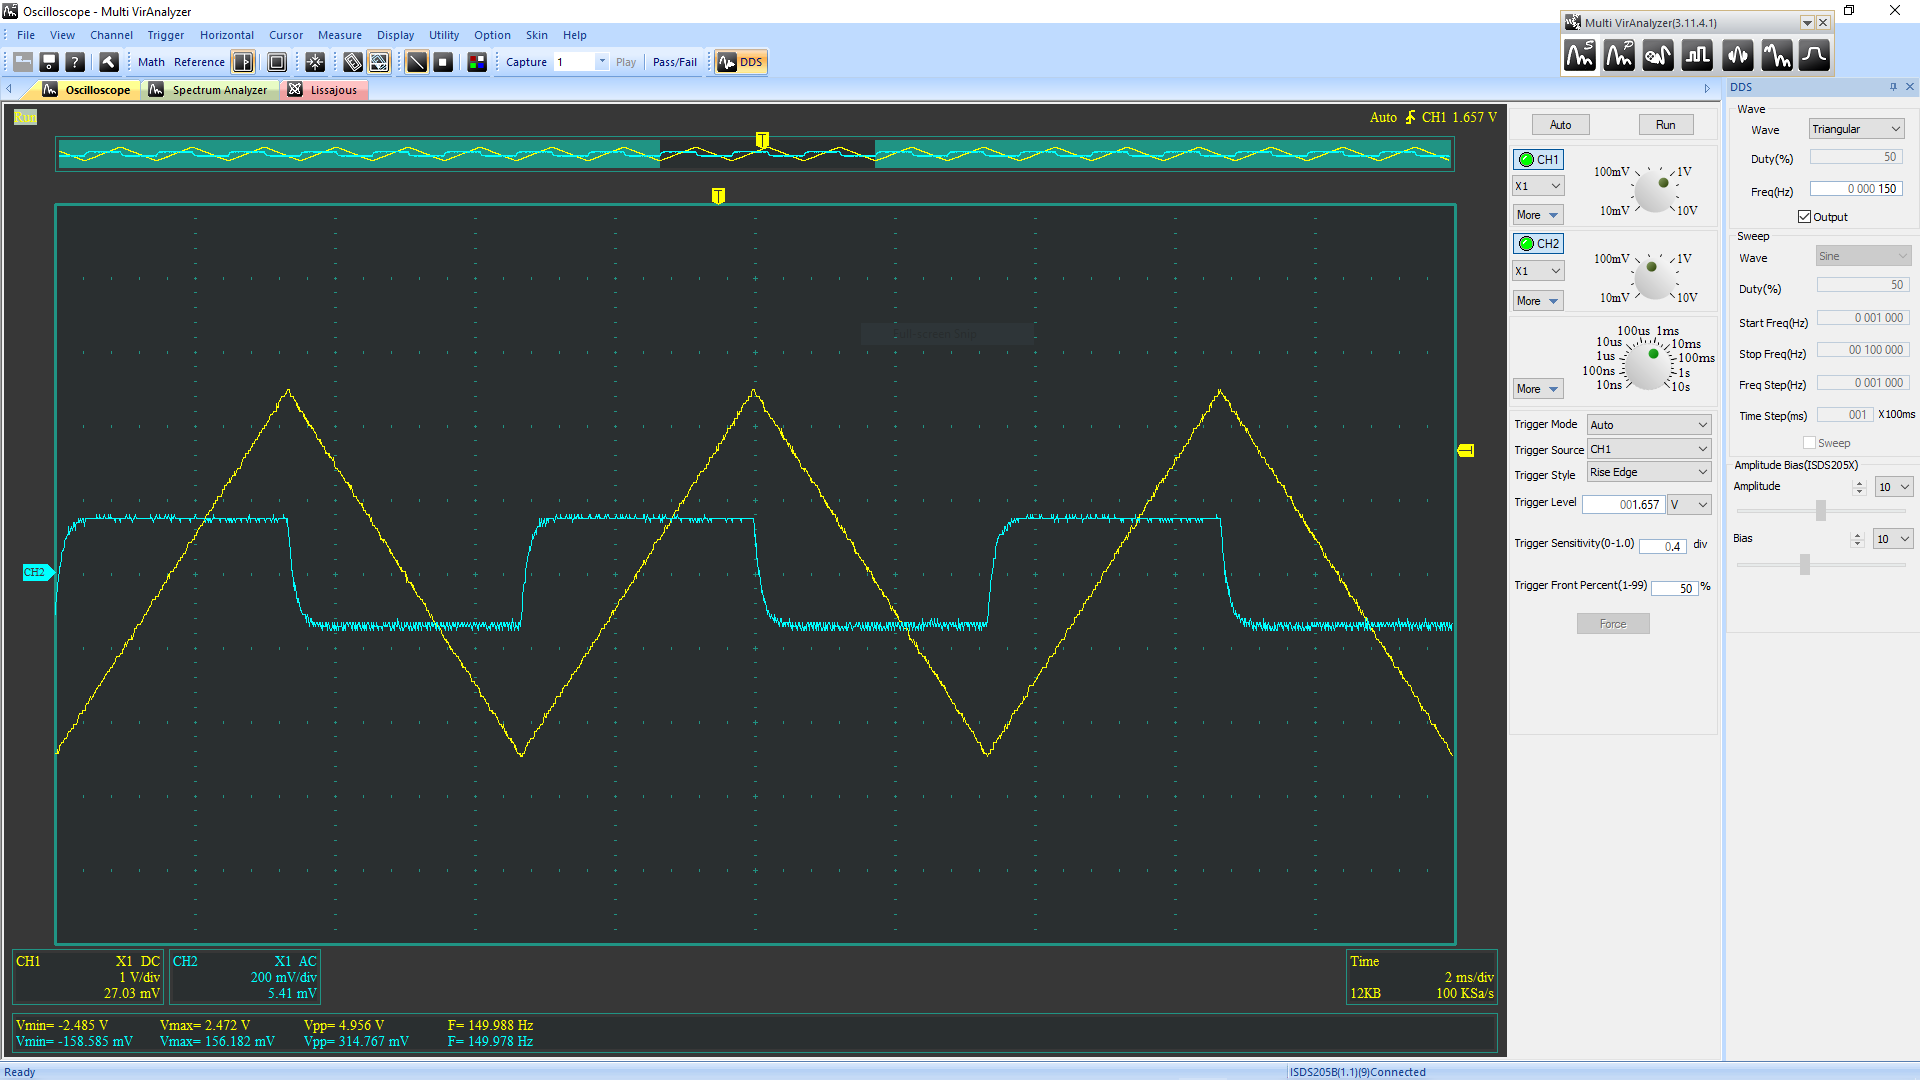
\includegraphics[width=\textwidth]{4.3.4.png}
        \caption{Waveform for part 4.3.4}
    \end{figure}
    \par For this part we are differentiating instead of integrating and this means we have to flip the component positions in the circuit. What this entails is that the frequency must be lowered in this case in order to attain the desired functionality. The output wave looks like a square wave and this is the correct output since the integral of the square wave was a triangle wave, the derivative of a triangle wave must be a square wave. The ratio of $ T / \tau $ in this case is,
    \[
        \frac{T}{\tau} = \frac{150}{1\times 10^{-4}} = 66.6667
    \]
    The ratio of $ V_{pp} / V_{rpp} $, in this case since the output voltage is across the resistor, would be,
    \[
        \frac{V_{pp}}{V_{rpp}} = \frac{4.956}{314.767 \times 10^{-3}} = 15.745
    \]
    \newpage
    \noindent 5.9
    \begin{center}
        \objects
            {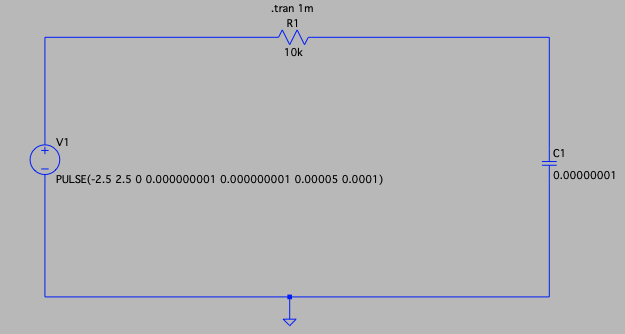
\includegraphics[width=0.85\textwidth]{4.3.1 LTSpice Circuit.png}}
            \:
            {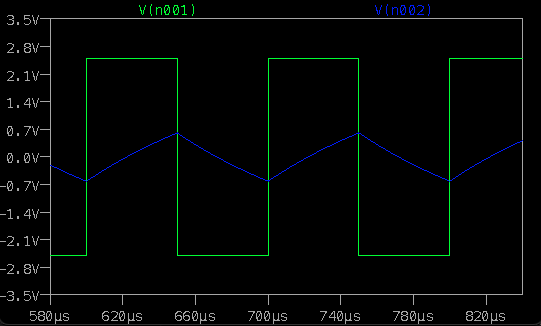
\includegraphics[width=0.85\textwidth]{4.3.1 LTSpice Output.png}}
    \end{center}
    \par The images above show the circuit and the output of the experiment conducted in 4.3.1. The circuit is a simple RC circuit with the resistor value being $ 10\ k\Omega $ and the capacitor being $ 0.01\ \mu F $. The function for the square wave is generated by built in "PULSE" function within LTSpice. It takes the arguments, from left to right, minimum and maximum voltage, rising and falling time, time on, and period of the wave. The rising and falling time of a square wave is essentially zero however, the program cannot take a zero input for this value. To combat this, the value is set to be very small compared to the time on and period of the function, here it is 1 ns. The period can be determined from the frequency set within the oscilloscope program, in this case 10000 Hz which makes the period 0.0001 s. Last is the time on parameter which can be determined using the duty cycle. Since the duty cycle is 50 \%, its value will just be half of the period, 0.00005 s. The output can be observed to be the same as that which is found experimentally.
    \newpage
    \begin{center}
        \objects
            {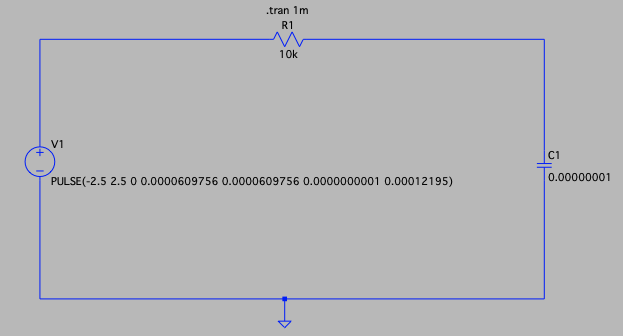
\includegraphics[width=0.95\textwidth]{4.3.2 LTSpice Circuit.png}}
            \:
            {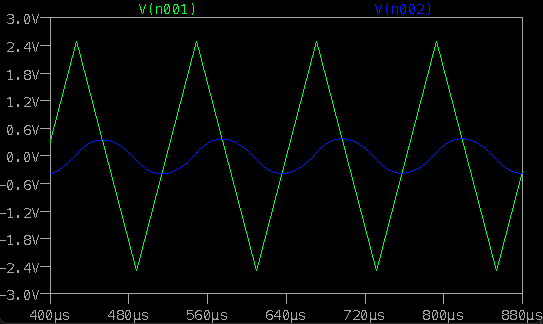
\includegraphics[width=0.95\textwidth]{4.3.2 LTSpice Output.png}}
    \end{center}
    \par This is the experiment setup of 4.3.2 and it is very similar to the previous setup. Here, the inputs to the PULSE function are changed since we require a triangular wave. The rising and falling time can be set to be half of the period. This will yield an equivalent time for which the function is rising and falling, equating to a triangular waveform. The period can be determined as before, from the frequency, and here the time on must be set to be very low since the time at on at the peak of a triangular wave is essentially zero. For this reason, here it is set to be 1 ns. All the other aspects of the circuit are the same and from the output, it can be seen that the expected behavior is observed. The integral of a triangular wave is a parabolic curve, and this is seen both experimentally and now as well in the simulation.
    \newpage
    \begin{center}
        \objects
            {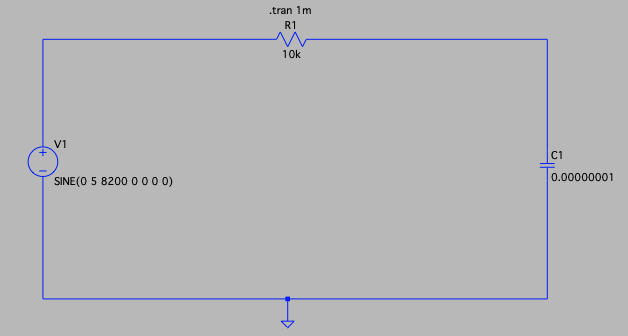
\includegraphics[width=0.95\textwidth]{4.3.3 LTSpice Circuit.png}}
            \:
            {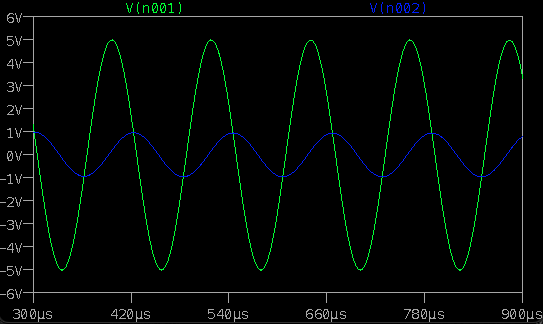
\includegraphics[width=0.95\textwidth]{4.3.3 LTSpice Output.png}}
    \end{center}
    \par This is the output and circuit for the experiment done in part 4.3.3, integration of the sine wave. Here, the voltage is defined by the "SINE" function which takes the inputs, DC offset, which is zero, amplitude which is 5, frequency which is 8200 from the oscilloscope program, and the rest deal with the angle offsets which are all zero. This give a sine wave which is seen in the output. The output voltage in blue is seen to be the integral of the sine wave, a cosine wave, which signifies the appropriate function of the circuit as it correlates to the results found experimentally.
    \newpage
    \begin{center}
        \objects
            {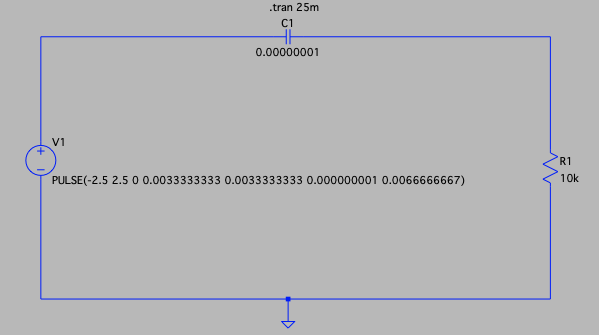
\includegraphics[width=0.95\textwidth]{4.3.4 LTSpice Circuit.png}}
            \:
            {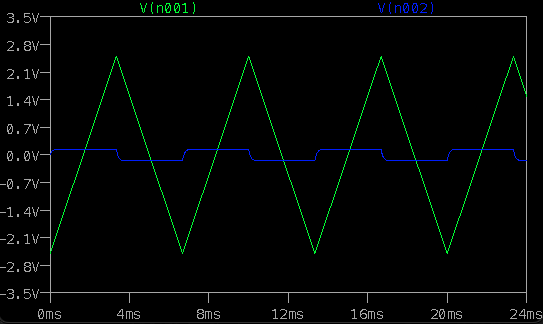
\includegraphics[width=0.95\textwidth]{4.3.4 LTSpice Output.png}}
    \end{center}
    \par For these next three experiments we are looking at the differentiation property of the RC circuit. Here, the triangular wave is defined similar to as it was previously only this time with a different frequency, 150 Hz. Since we are looking at differentiation, the component locations are switched and the output voltage is being measured across the resistor. The output can be seen to be a square wave which is the expected behavior and the same is found experimentally.
    \newpage
    \begin{center}
        \objects
            {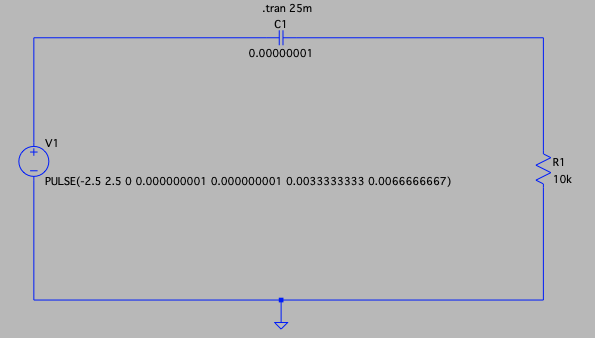
\includegraphics[width=0.95\textwidth]{4.3.5 LTSpice Circuit.png}}
            \:
            {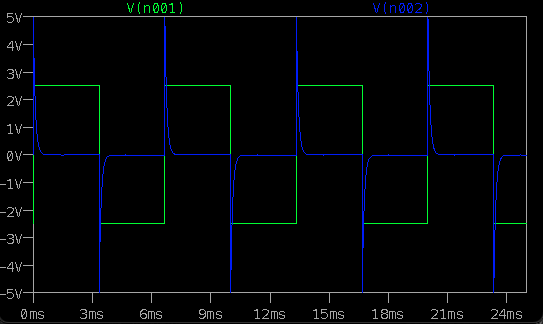
\includegraphics[width=0.95\textwidth]{4.3.5 LTSpice Output.png}}
    \end{center}
    \par This is the graph of the derivative of the square wave and it too matches up with the results found experimentally. The input wave is defined the same as before, this time with the frequency again being 150 Hz. The result is a curve with discontinuities at the vertices of the square and this makes sense since the derivative at a point does not exist. The same result is found in the experimental waveform, verifying both results.
    \newpage
    \begin{center}
        \objects
            {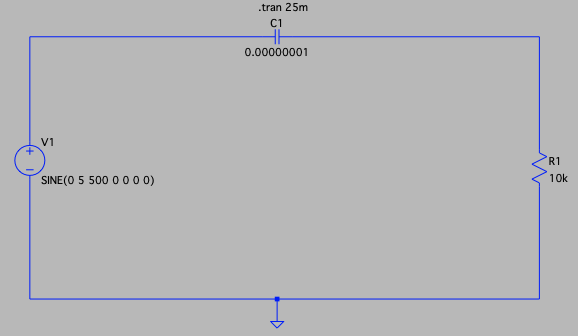
\includegraphics[width=0.95\textwidth]{4.3.6 LTSpice Circuit.png}}
            \:
            {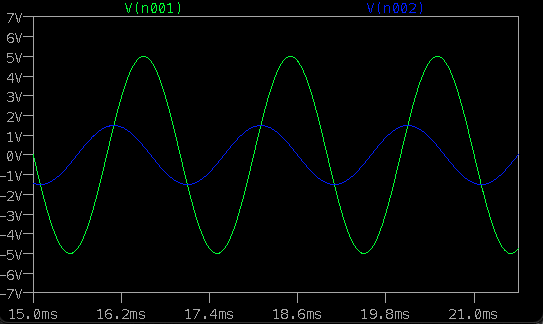
\includegraphics[width=0.95\textwidth]{4.3.6 LTSpice Output.png}}
    \end{center}
    \par Finally, for the last experiment, we have the derivative of the sine wave. Here the input wave is defined as before but this time with a frequency of 500 Hz. The component values are the same as they have been and the result is observed to be a cosine wave which is expected. This result was also found experimentally, verifying both results.
\end{document}
